\chapter{Cooling and Trapping in a MOT}
\section{Chapter Outline}
This chapter presents a description of the components of the experiment which are used to trap and cool atoms in a \ac{mot}. 
\section{The Navigator Vacuum Chamber}\label{sec:vacuum_chamber}
The vacuum chamber, along with the components mounted to it, make up the majority of the hardware used in the preliminary trapping and cooling stages of the experiment. The chamber is made of 316L stainless steel which helps to minimise the influence of stray magnetic fields that could otherwise affect the performance of the \ac{mot}. The chamber contains 16 DN40 ConFlat ports arranged on the edges of three octagons, one in each cartesian coordinate plane. Six of these ports are used to provide optical access for the 3D \ac{mot}, and a further four are used to connect to the 2D \ac{mot} system, a gate valve, the NexTorr pump and to provide power to the in-vacuum 3D \ac{mot} coils. Two of the remaining ports are used to provide optical access for the imaging systems --- a CCD camera and a photodiode --- or a microwave horn, depending on the specific experiment. The last four ports are not used for additional optical access since their line of sight to the atoms is obscured by the \ac{mot} coils. Two DN63 ports lie along one axis, which is conventionally taken to be the \(x\) axis. These ports are used to mount the optics for driving Raman transitions and as such, defines the axis along which the atom interferometer is sensitive to accelerations\footnote{For more information about the Raman optical system, refer to \SectionRef{sec:setup_ramanoptics}}. \par\noindent
A diagram of the vacuum chamber and the main \ac{mot} components is shown in \FigureRef{fig:mot_system}. The chamber is pumped down to a pressure of around \pow{5}{-10}\sivalue{}{\milli\bar} using a NexTorr D100-5 pump. This is a composite system consisting of \ac{neg} and an ion pump. The \ac{neg} is a porous sintered zirconium (St 172) element, which reacts with chemicals such as hydrogen, water, nitrogen, oxygen and hydrocarbons. Most of these were removed during the initial baking and roughing pump stages. Under \ac{uhv} conditions, the largest contributor to the pressure is hydrogen which the \ac{neg} can pump at a speed of \sivalue{100}{\litre\per\second}. Any species that are not absorbed by the \ac{neg}, in particular Rubidium, are pumped by the \sivalue{5}{\litre\per\second} ion pump.
\begin{figure}
    \centering
    \def\svgwidth{1\textwidth}
    \input{Figures/Chapter4/Vacuum.pdf_tex}
    \caption[\ac{mot} system component diagram]{A diagram of the main components on the vacuum chamber used for the \ac{mot} systems. Rubidium atoms are dispensed and loaded into the 2D \ac{mot} before being pushed into the main chamber and collected in the 3D \ac{mot}. A set of 6 beam collimators provide the light necessary to slow and cool atoms, which are trapped using the spherical quadrupole field generated by the illustrated coils. Not shown are additional bias coils along each \ac{mot} beam axis to null stray fields at the centre of the chamber.}
    \label{fig:mot_system}
\end{figure}   
\subsection{The 2D MOT system}\label{sec:2d_mot}
Initially, atoms were loaded into the 3D \ac{mot} from a background vapour. Whilst this was a relatively simple scheme, a very high partial pressure of Rubidium is required to achieve a fast loading rate (see \SectionRef{subsec:loading_rate}). However, this was undesirable from the point of view of the atom interferometer, as it would result in a poor fringe contrast due to collisions with background atoms and a worse signal to noise ratio, i.e. the ratio of the number of atoms in the interferometer to the total number of detected atoms. Replacing the source of atoms for the 3D \ac{mot} with a side-arm to function as a 2D \ac{mot}~\cite{Dieckmann1998} satisfied the two requirements of a fast loading rate and low base pressure in the main chamber. \par\noindent
A diagram of the setup required to produce a 2D \ac{mot} is presented in~\FigureRef{fig:2d_mot_diagram}. It is similar to the 3D \ac{mot}, with the main exception being that only 4 beams are used to cool the atoms along 2 orthogonal axes. In addition to this, its design is focused towards the production of a large flux of cold atoms which can be subsequently loaded into a 3D \ac{mot}. For instance, the beams used to cool the atoms are collimated to a large waist size and the coils are designed to give a cylindrical quadrupole field with a line of zero magnetic field along the axis of symmetry. Along this axis, the atoms are free to move which results in an atomic beam. To improve the collimation of this atomic beam, a larger radial field gradient than usually used in a 3D \ac{mot} system is used to increase the radial confinement of atoms. In addition, a pinhole is placed at the exit of the cell, so that atoms with a high radial velocity component will miss the aperture. This pinhole also greatly reduces the conductance between the 2D \ac{mot} cell and the main chamber, which means that a comparatively high background pressure (hence, loading rate) can be maintained in the 2D \ac{mot} cell, without greatly increasing the pressure in the main chamber. The pinhole is drilled into a silicon plate, which is used to partially reflect a beam that propagates along the central axis. This creates an unbalanced molasses that cools atoms with a large axial velocity and due to the differing radiation pressure, pushes atoms out through the pinhole. By slowing a larger proportion of atoms to within the capture velocity of the 3D \ac{mot} and not solely relying on diffusion of the atoms, this configuration, often referred to as a \(2D\+\) \ac{mot}, loads a 3D \ac{mot} faster than the 4-beam counterpart. \par\noindent 
A schematic of the optical components for the 2D \ac{mot} is presented in~\FigureRef{fig:2d_mot}. The cooling light originates from a single fibre, which is collimated using two aspheric lenses to a beam waist of \sivalue{9.5}{\milli\metre} and linearly polarised before being evenly split into two beams using a \ac{hwp}, one for each cooling axis. Each beam passes through a beam-splitter and prism pair, to increase the volume covered by the 2D \ac{mot} beams and is circularly polarised by a pair of \ac{qwp} before entering the \ac{ar} coated glass cell. On the opposing side of the cell, a \(\sivalue{25}{\milli\metre} \times \sivalue{35}{\milli\metre}\) retro-reflecting mirror is used to provide the counter-propagating \ac{mot} beam. This is coated with a layer of quartz to form a \ac{qwp}, so that the reflected beam has the required polarisation for cooling atoms along that axis. The push beam is created using a second fibre input and a fixed collimator to give a beam waist of \sivalue{1.5}{\milli\metre}. This is mounted onto a \sivalue{1}{\inch} kinematic mount so that the alignment of the push beam with respect to the \sivalue{0.7}{\milli\metre} pinhole at the other end of the cell can be optimised. A linear polariser is placed here to reduce the effect of polarisation drift on the axial cooling of the 2D \ac{mot}. The cell, manufactured by ColdQuanta, has dimensions of \(\sivalue{30}{\milli\metre} \times \sivalue{30}{\milli\metre} \times \sivalue{44}{\milli\metre}\) and is specifically designed for creating a 2D\+ \ac{mot} and contains two rubidium dispensers composed of rubidiumchromate (RbCrO\(_4\)) and a reducing agent. These were activated by passing a large current through them to remove a thin oxidation layer. To produce rubidium, a current is passed through the dispenser to trigger an electro-chemical reduction reaction. The reducing agent also acts to sorb the unwanted products, so that they do not contaminate the cell and only rubidium evaporates from the dispenser. \par\noindent
The cylindrical quadrupole field is generated by a set of coils that are manufactured by ColdQuanta. Their geometry is such that the axis of zero magnetic field coincides with the central longitudinal axis of the source cell. Each coil contains {\textbf {x}} number of turns and produces a radial field gradient per current of {\textbf {20}}\;\sivalue{}{\gauss\per\centi\metre\per\ampere}. A simulation of the field gradient along each axis, along with the magnetic field in each plane of symmetry is shown in \FigureRef{fig:2d_mot_field_gradient}, which indicates that the field gradient is very uniform across the centre of the cell. In addition to this, each \ac{mot} axis has a separately controlled pair of coils in a Helmholtz configuration to provide a bias field that cancels nulls the field along the 2D \ac{mot} axis. These coils are made of 20 turns of wire that has a core diameter of \sivalue{1}{\milli\metre}, which gives a field per current of {\textbf{z}}\;\sivalue{}{\gauss\per\ampere}.
\begin{figure}
    \centering
    \def\svgwidth{\columnwidth}
    \subfloat[][]{\scalebox{0.3}{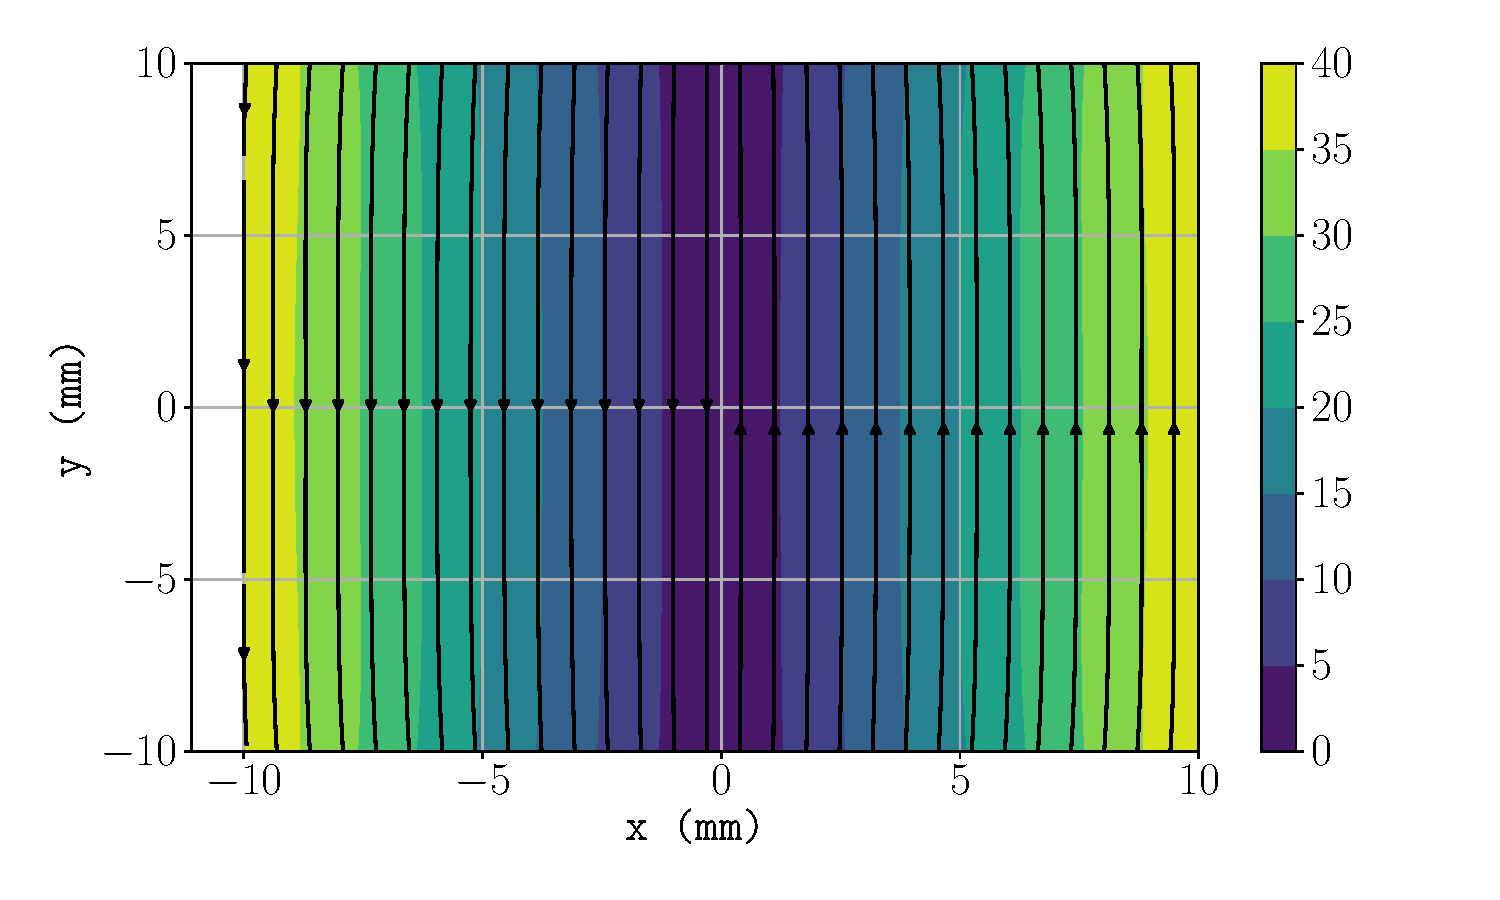
\includegraphics{2D_field_xy.pdf}\label{fig:label}}}
    \subfloat[][]{\scalebox{0.3}{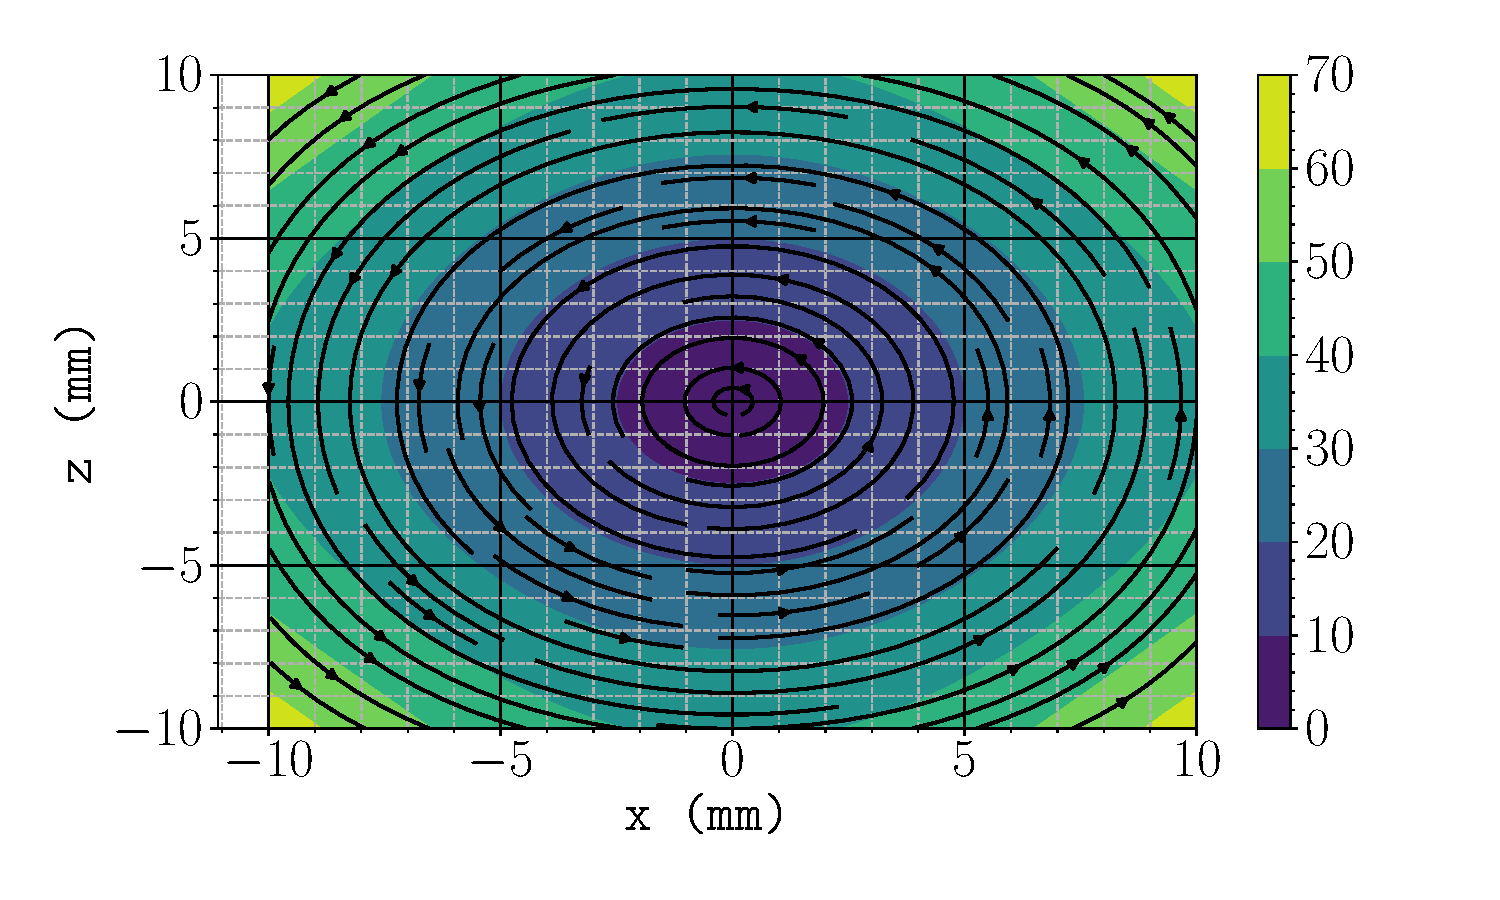
\includegraphics{2D_field_xz.pdf}}\label{fig:label}}\\
    \subfloat[][]{\scalebox{0.3}{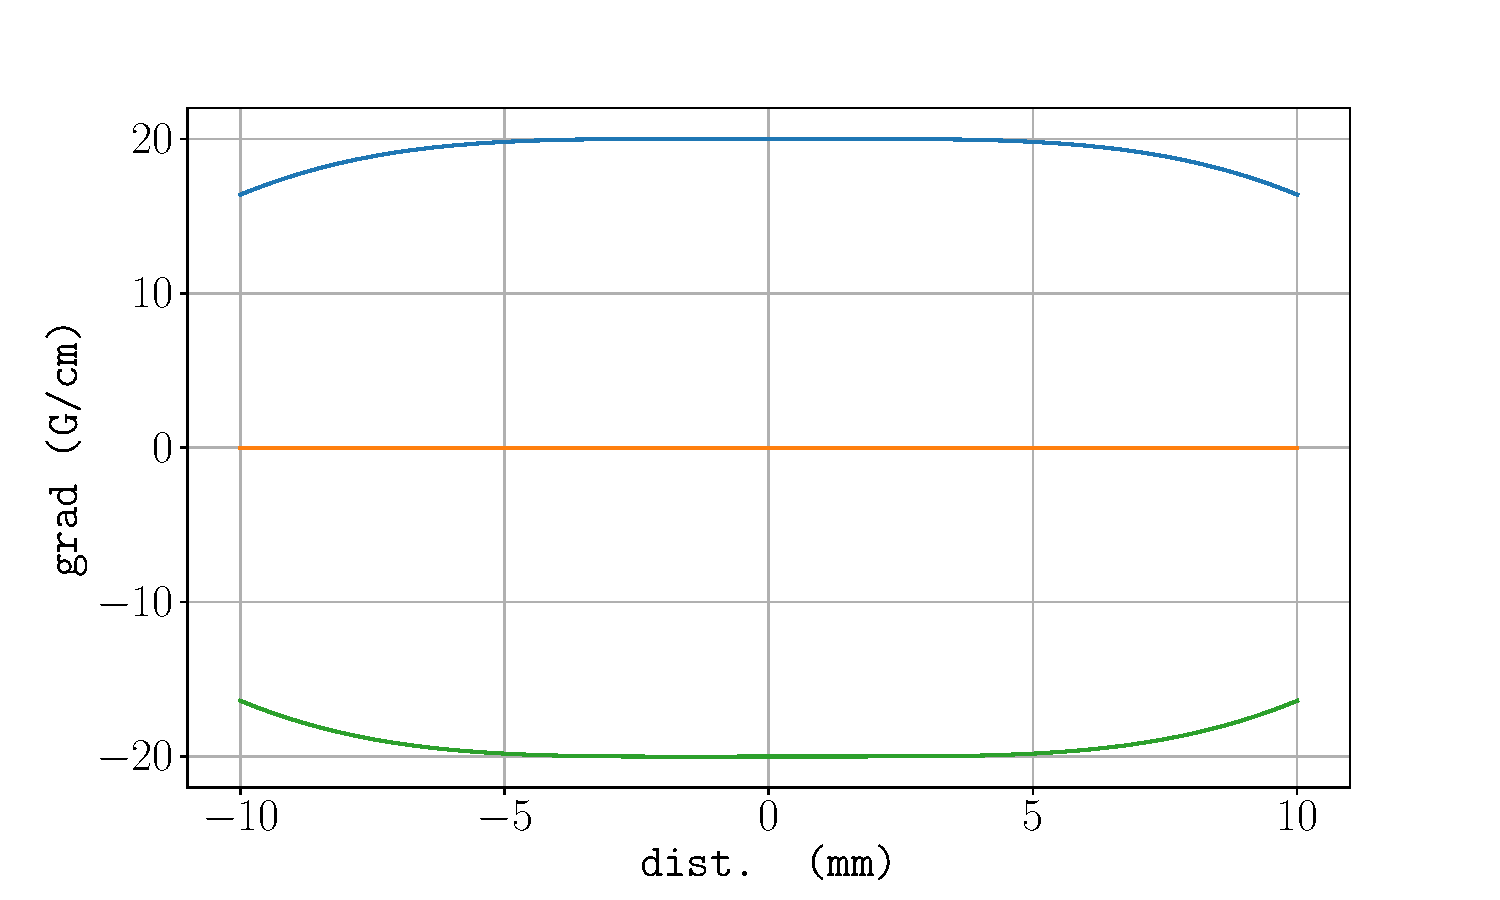
\includegraphics{2D_grad.pdf}}\label{fig:label}}
    \caption[Simulated field and field gradients for the 2D \ac{mot} quadrupole coils]{Simulated field and field gradients for the 2D \ac{mot} quadrupole coils. In this coordinate system, the 2D \ac{mot}cools and traps atoms in the \(\vec{x}\) and  \(\vec{z}\) directions. The simulation was performed using a nominal current of \sivalue{1}{\ampere}, which corresponds to a current density in each coil of \sivalue{7.78}{\ampere\per\square\milli\metre}. The magnitude of the magnetic field (in units of \sivalue{}{\gauss}) and its direction in the axial and radial planes of symmetry are shown in \textbf{(a)} and \textbf{(b)}, respectively. \textbf{(c)} shows the field gradient components \(\partial_x B_x\) (blue), \(\partial_y B_y\) (orange) and \(\partial_z B_z\) (green) along their corresponding axes.}
    \label{fig:2d_mot_field_gradient}
\end{figure}
\subsection{The 3D MOT system}\label{sec:3d_mot}
The main chamber contains the apparatus that is used to make a 3D \ac{mot}. A diagram of the optical and magnetic fields used to create this \ac{mot} is presented in~\FigureRef{fig:3d_mot}. Each \ac{mot} beam is created using a collimator as shown in~\FigureRef{fig:mot_collimator}. Light enters through a \ac{pm} fibre using an FC/APC connector and is collimated using a \sivalue{75}{\milli\metre} focal length lens to give a collimated beam with a waist size of around \sivalue{7.5}{\milli\metre}. At the output of each collimator is a \ac{qwp}, with its slow axis oriented at a 45\(^\circ\) angle to the fast or slow axis of the fibre, depending on the particular collimator, to produce either left- or right-handed circularly polarised light. The \ac{mot} beams are oriented so that their intersection is at the centre of origin of a cartesian coordinate system. Since the \ac{mot} forms at the position where the magnetic field is zero, this system is set up so that beams overlap at the centre of the chamber, which is equidistant from each \ac{mot} coil. The \ac{mot} beams along the axial direction of the quadrupole field (conventionally referred to as the \(\vec{z}\) direction) are orthogonally polarised to the others along the \(\vec{x}\) and \(\vec{y}\) directions. This takes into account of the different direction of the magnetic field gradient along each axis (see below), so that the polarisation of each \ac{mot} beam is such that an atom moving away from the centre of the trap is slowed and optically pumped into a state which feels a conservative potential.
\subsubsection{Spherical quadrupole magnetic field}
The magnetic field for the 3D \ac{mot} is created by a pair of coils in an anti-Helmholtz configuration. Along the axis of symmetry, the magnetic field from a current-carrying loop is given by the Biot-Savart law. {\textbf{Some description of the spherical quadrupole field}}.
Each coil consists of rectangular wire coated in a \sivalue{35}{\micro\metre} thick layer of Pyre-M.L, a UHV-compatible polyamide which provides a layer of insulation between each loop. The wire has a cross-section of dimensions \(\sivalue{1.1}{\milli\metre} \times \sivalue{1.1}{\milli\metre}\), with 20 axial loops and 12 radial loops. The inner diameter of the coil is \sivalue{25.4}{\milli\metre}, to allow for optical access of the \(\vec{z}\)-axis \ac{mot} beams, and the maximum diameter is \textbf{59.2}\sivalue{}{\milli\metre} -- small enough that the coil could be inserted into the chamber through the DN63 CF ports. The coils are mounted to the chamber using groove grabbers which clamp into grooves inside the wall of the DN40 ports.  The formers are designed to maximise the surface area between them and the chamber, which in turn aims to maximise the rate at which heat is dissipated from the coils. Once mounted, the distance between the innermost loops is \sivalue{70}{\milli\metre}. \FigureRef{fig:mot_coil_plots} shows the magnetic field, measured using a Hall probe, along the axis of symmetry for each of the coils with a current of \sivalue{2.53}{\ampere}. In addition to this, the field and corresponding axial field gradient when the coils are separated by \sivalue{70}{\milli\metre} is shown in \FigureRef{fig:mot_coil_gradient}. This is in close agreement with the value expected from simulating the field produced by the coils - the magnetic field in the axial and radial planes of symmetry and shown in~\FigureRef{fig:3D_mot_axial} and~\FigureRef{fig:3D_mot_radial}, respectively.
\begin{figure}
    \centering
    \def\svgwidth{\columnwidth}
    \subfloat[][]{\scalebox{0.3}{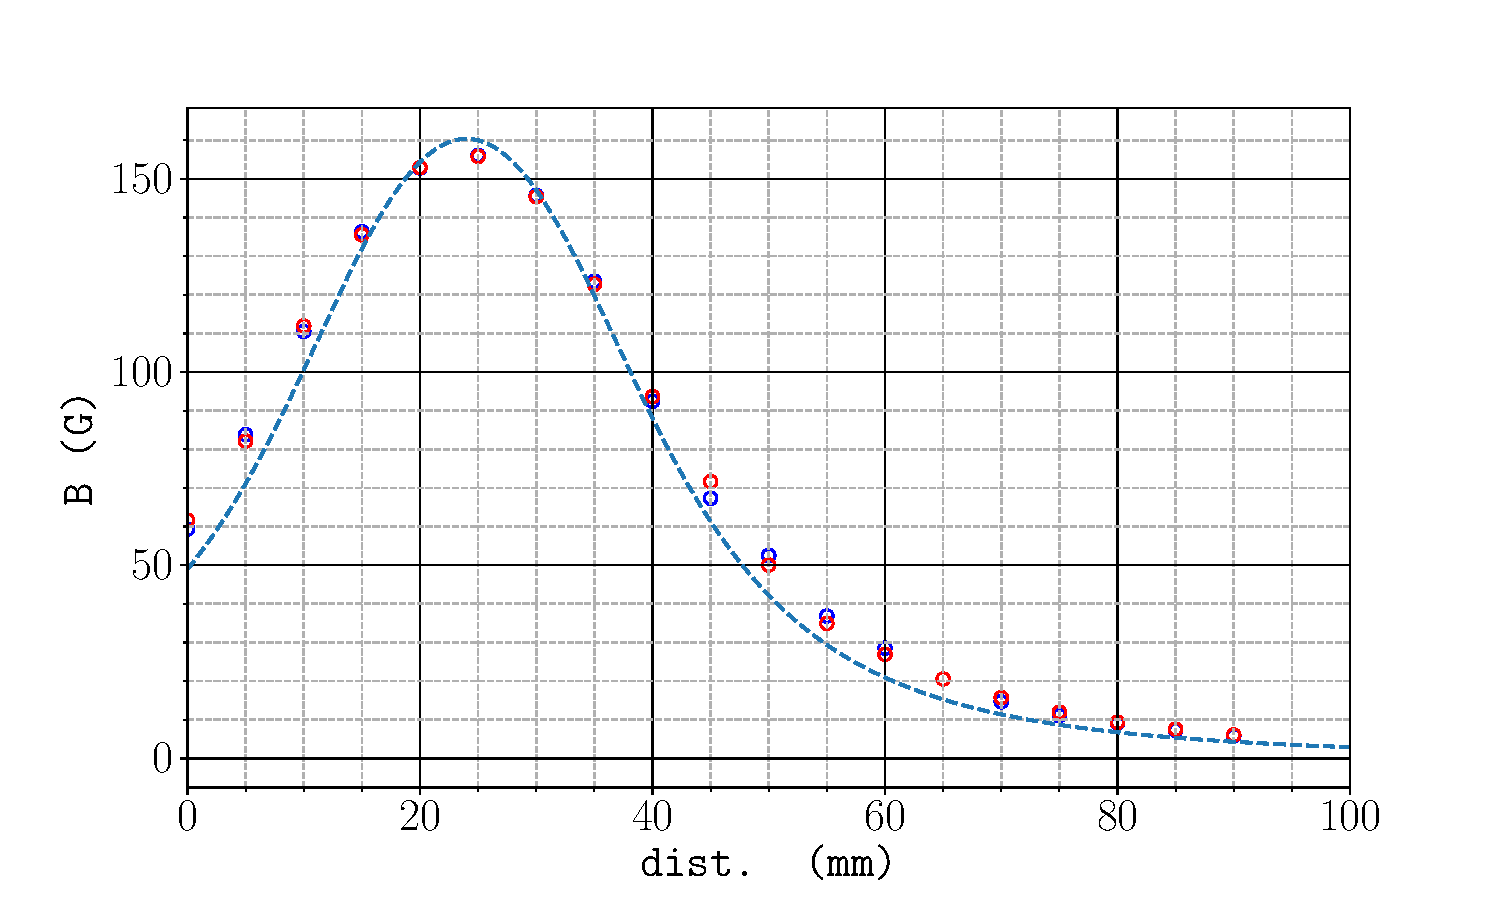
\includegraphics{mot_field_3D.pdf}\label{fig:mot_coil_plots}}}
    \subfloat[][]{\scalebox{0.3}{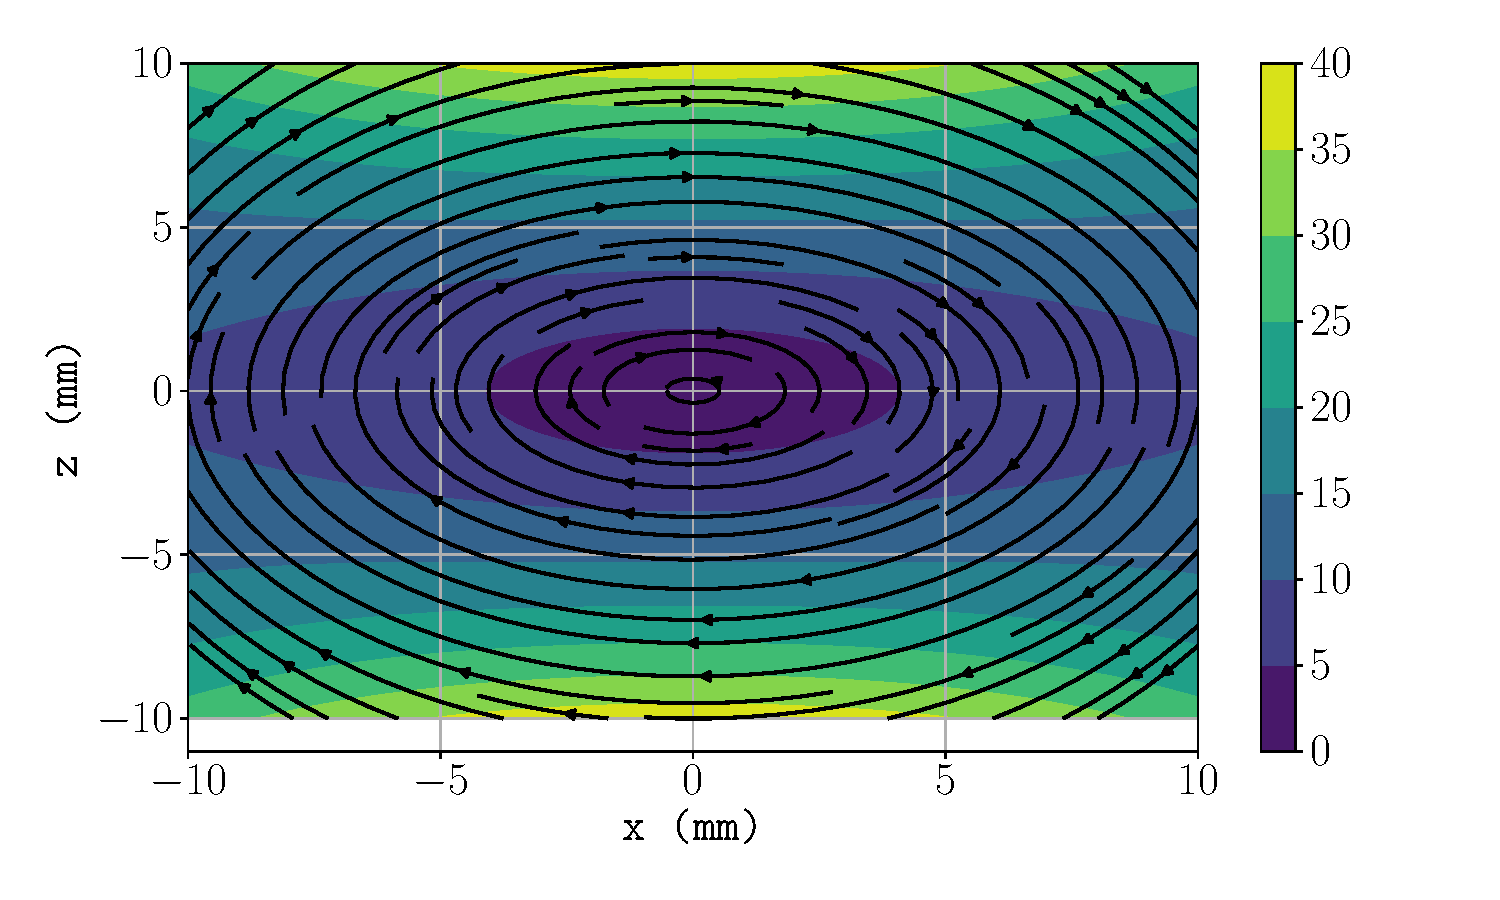
\includegraphics{3D_field_xz.pdf}}\label{fig:mot_coil_gradient}}\\
    \caption[Measured magnetic field and field gradient for the 3D \ac{mot} coils]{Measured magnetic field and field gradient for the 3D \ac{mot} coils. \textbf{(a)} shows the axial magnetic field for the two coils as measured using a Hall probe. The dashed line is the axial field as calculated from the simulation shown in~\FigureRef{fig:3D_mot_field_sim}.}

    \label{fig:3D_mot_field_measured}
\end{figure}
\begin{figure}
    \centering
    \def\svgwidth{\columnwidth}
    \subfloat[][]{\scalebox{0.3}{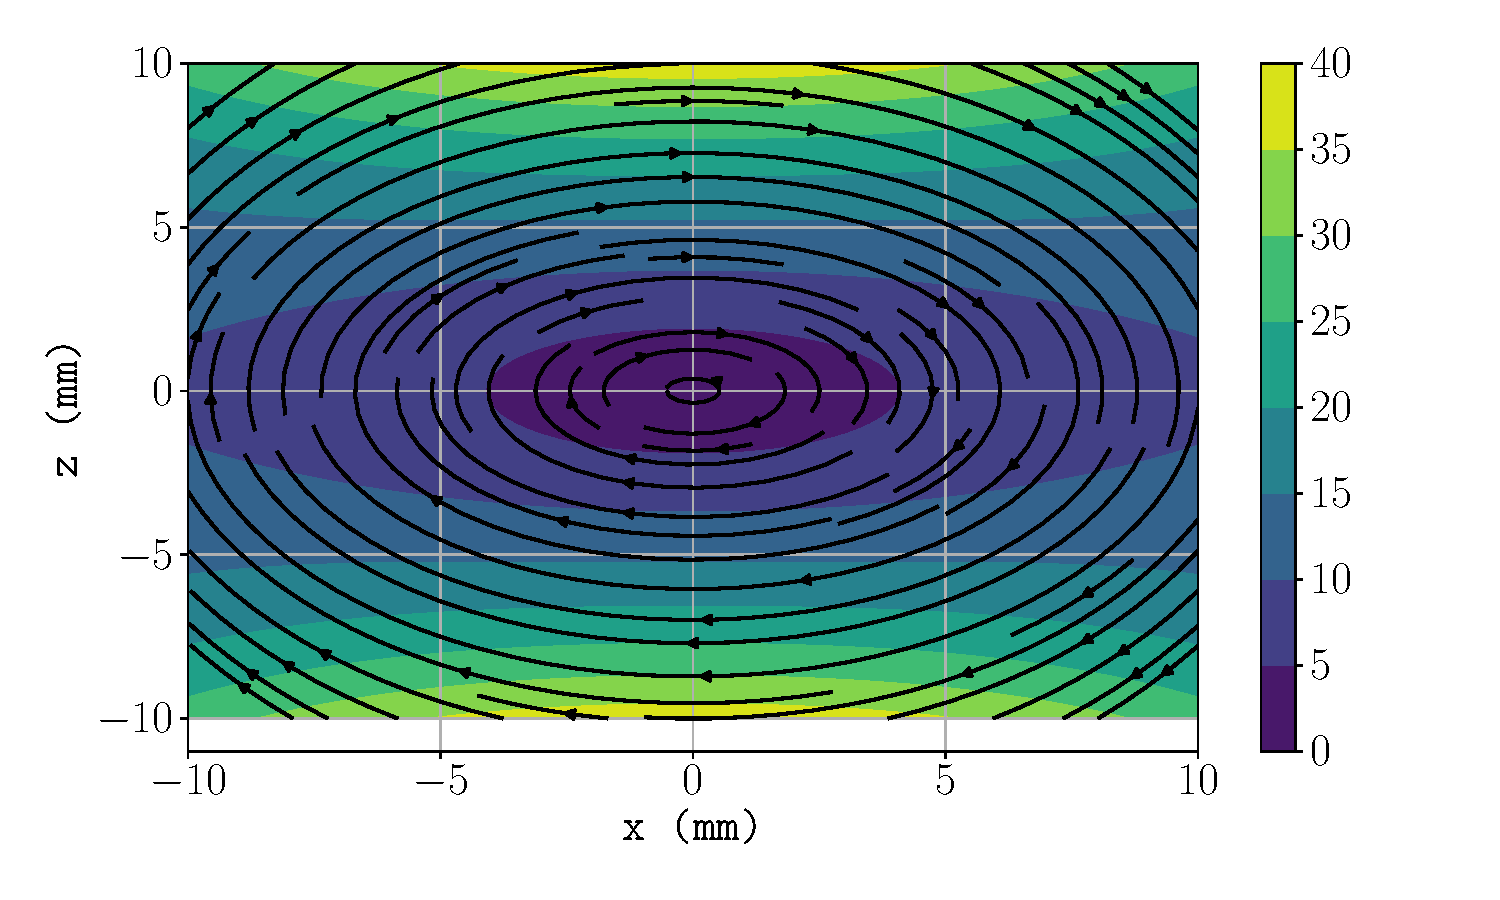
\includegraphics{3D_field_xz.pdf}}\label{fig:3D_mot_axial}}
    \subfloat[][]{\scalebox{0.3}{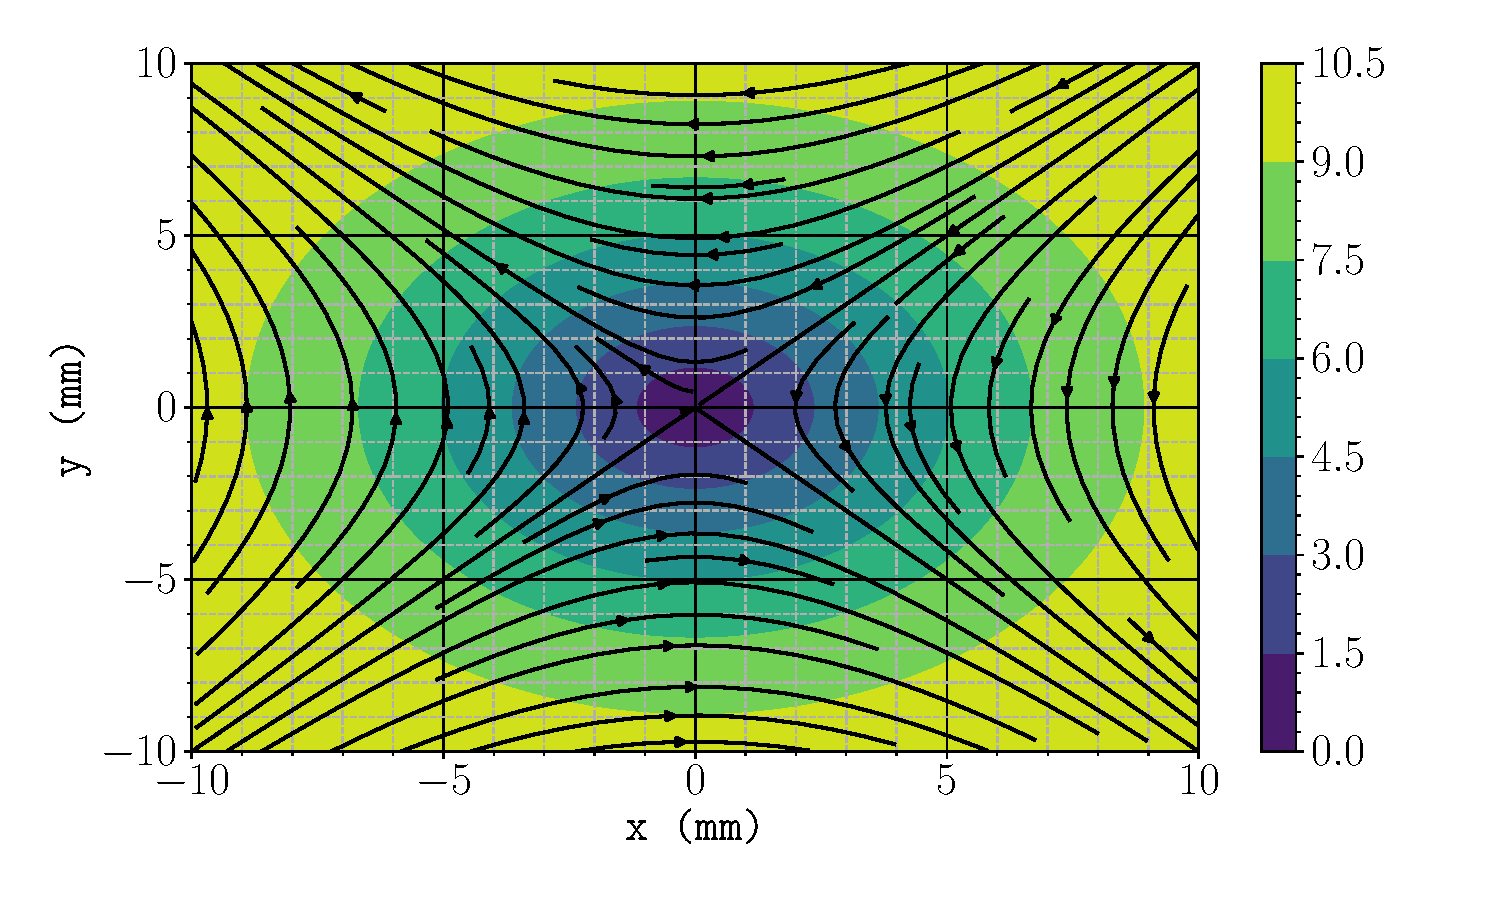
\includegraphics{3D_field_xy.pdf}\label{fig:3D_mot_radial}}}\\
    \caption[Simulated magnetic field for the 3D \ac{mot} quadrupole coils]{Simulated magnetic field for the 3D \ac{mot} quadrupole coils. In this coordinate system, the axial direction is defined as the \(\vec{z}\) axis. The simulation was performed using a nominal current of \sivalue{2.53}{\ampere}, which corresponds to a current density in each coil of \sivalue{1.33}{\ampere\per\square\milli\metre}. The magnitude of the magnetic field (in units of \sivalue{}{\gauss}) and its direction in the axial and radial planes of symmetry are shown in \textbf{(a)} and \textbf{(b)}, respectively.}
    \label{fig:3D_mot_field_sim}
\end{figure}
\subsubsection{Bias Coils}
Three orthogonally arranged pairs of Helmholtz coils are used during the experiment to null the magnetic field at the centre of the chamber. This is required for strong sub-Doppler cooling of the atom cloud in an optical molasses  where the presence of a magnetic field reduces the cooling efficiency~\cite{Walhout1992}. These coils are also used in subsequent stages of the experiment to provide a bias field along the appropriate axes during state preparation, interferometry and state detection. Each coil was wound using \sivalue{1}{\milli\metre} thick wire and consisted of 5 axial and 10 radial turns. For a pair of coils in Helmholtz configuration, the magnetic field gradient at the centre is minimised when the axial separation \(a\) is equal to the coil radius \(r\), but the geometry of the vacuum chamber meant that it was not possible to satisfy this condition. The radii and axial separations of each coil pair is presented in \TableRef{tab:bias_coils}.\begin{table}
    \begin{tabular}{|c|c|c|c|c|}
        \hline
        Axis & \(a\) (mm) & \(r_i\) (mm) & \(r_o\) (mm) \\
        \hline 
        \(\vec{x}\) & 88& 105 & 115 \\
        \(\vec{y}\) & 132 & 178 &188\\
        \(\vec{z}\) & 116& 123&133 \\
       \hline 
\end{tabular}
\caption[Table of parameters for each 3D \ac{mot} bias coil.]{Table of parameters for each 3D \ac{mot}bias coil. \(a\) denotes the axial separation between each coil, \(r_i\) and \(r_o\) are the inner and outer radi. Each coil was wound to give 50 loops (5 axial and 10 radial turns).}
\label{tab:bias_coils}
\end{table}
\subsection{CCD Imaging}\label{sec:imaging}
The characterisation of the \ac{mot} stage of the experiment was achieved using a CCD camera to spatially resolve the atom cloud by detecting light emitted from the atoms during resonance fluorescence. Measuring the spatial distribution of atoms is useful, for example in estimating the temperature of the cloud by measuring the rate of thermal expansion. \FigureRef{fig:imaging_optics} shows a diagram of the apparatus used for imaging. A pair of \sivalue{125}{\milli\metre} and \sivalue{50}{\milli\metre} focal length lenses are used to image the cloud onto a Pike F505-B CCD camera, which has a maximum resolution of \(2452 \times 2054\) pixels. The pixel size in the object plane was measured by placing a ruler in that plane, giving a calibration factor of \sivalue{5.1}{pixel\per\milli\metre}. A bandpass filter is placed between the lens and the CCD which transmits \sivalue{780}{\nano\metre} light at an efficiency of 60\% and blocks background light at other wavelengths. 
\begin{figure}
    \centering
    \def\svgwidth{
    0.6\textwidth}
    \input{Figures/Chapter4/ccd_optics.pdf_tex}
    \caption[Optical setup for CCD imaging]{Optical setup for CCD imaging. Two lenses are used to magnify the image of the atom cloud on the CCD. A bandpass filter is placed in front of the sensor to block out backgound light at wavelengths other than \sivalue{780}{\nano\metre}. All lengths are given in millimetres.}
    \label{fig:imaging_optics}
\end{figure}
\par\noindent
An estimate of the number of atoms \(N_a\) can determined by relating the incident optical power \(P_\textnormal{ccd}\) to the scattering rate per atom as follows
\begin{equation}
    P_\textnormal{ccd} = \frac{\Omega}{4\pi}  R_\textnormal{sc}  \hbar \omega N_a
\end{equation}
where $\Omega/4\pi = \textbf{x}\sivalue{}{\steradian}$ is the fractional solid angle subtended by the imaging optics, \(R_\textnormal{sc}\) is the scattering rate as previously defined in~\EquationRef{eq:scattering_rate} and \(\hbar \omega = \sivalue{1.6}{\electronvolt}\) is the emitted photon energy. This incident power is then related to the integrated number of pixel counts \(C_\textnormal{int}\) by 
\begin{equation}
    C_\textnormal{int} = \alpha \tau_\textnormal{exp} \eta P_\textnormal{ccd}
\end{equation}
where \(\tau_\textnormal{exp}\) is the exposure time, \(\eta = 0.14\) is the quantum efficiency of the CCD and \(\alpha\) is a scaling factor that relates the total charge collected to the total number of pixel counts. By varying the exposure time used to image a collimated beam with a total power of \sivalue{0.17}{\micro\watt}, the total number of counts recorded by the camera as a function of exposure time is plotted in~\FigureRef{fig:camera_counts}. This gives a count scaling factor of \(\alpha\) = \pow{2.2}{5}\,counts\,\sivalue{}{\per\micro\second\per\micro\watt}.
\begin{figure}
    \centering
    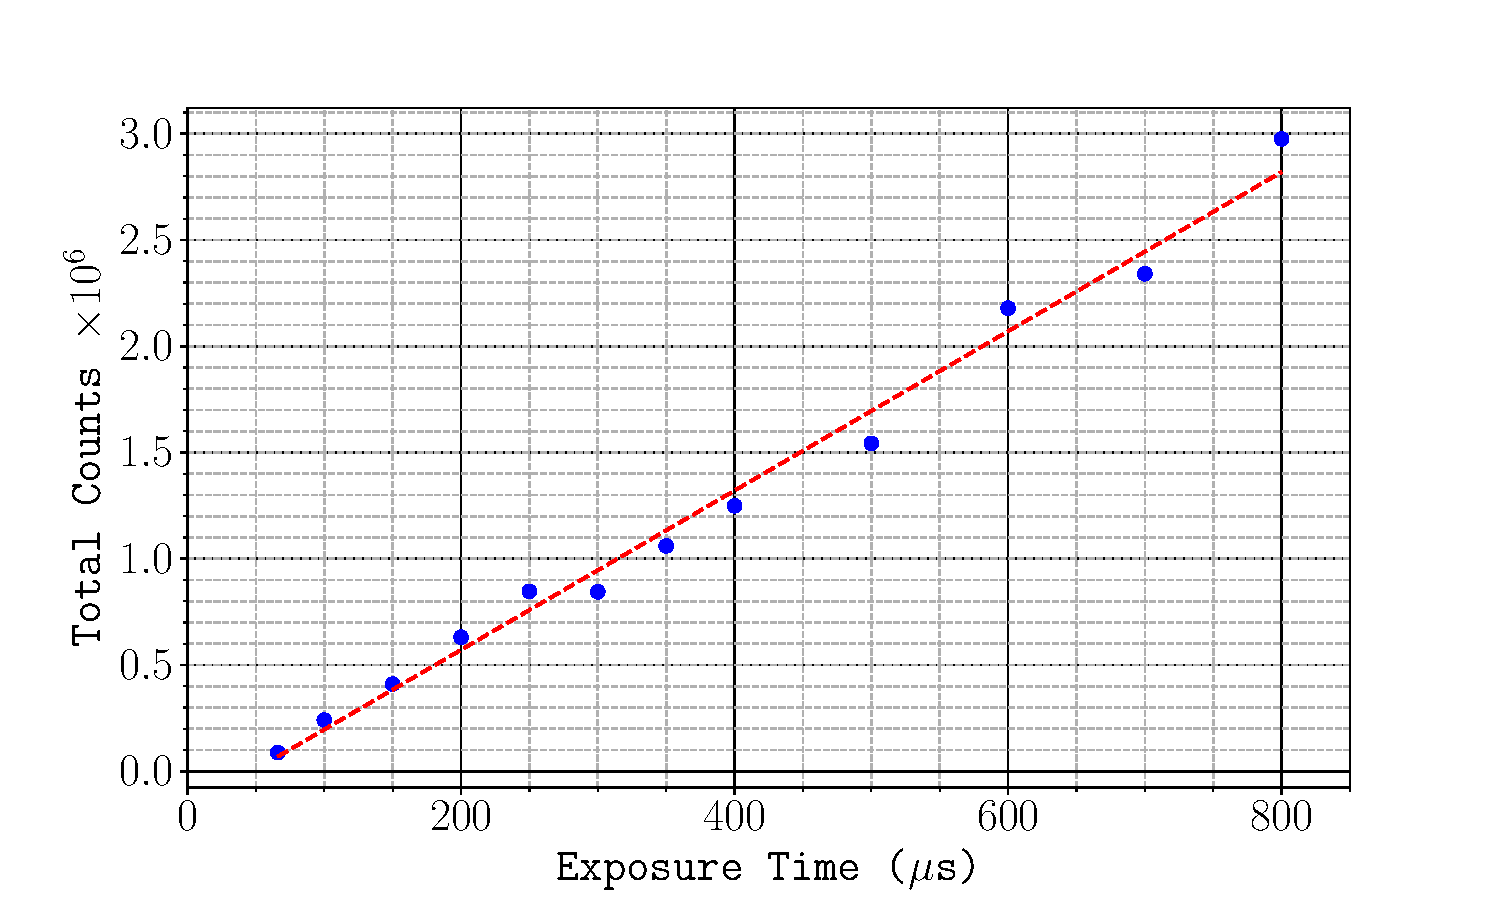
\includegraphics[width=0.5\textwidth]{cam_per_exposure}
    \caption[Integrated pixel counts as a function of CCD exposure time.]{Integrated pixel counts as a function of CCD exposure time for an incident optical power of \sivalue{0.17}{\micro\watt}. The dashed line indicates a linear regression which gives a scaling factor of \(\alpha\) = \pow{2.2}{5}\,counts\,\sivalue{}{\per\micro\second\per\micro\watt}.}
    \label{fig:camera_counts}
\end{figure}
\section{Generating MOT light}
\subsection{Muquans Laser Control}
\subsubsection{Frequency Control}
\subsubsection{Real-Time Communication} \label{subsec:muquans_comm}

\section{Controlling the MOTs}
\subsection{Optical Fibre Network}
\subsection{Magnetic Field Control}

\section{Characterising the 3D MOT}
\subsection{3D MOT Loading Rate}\label{subsec:loading_rate}
\subsection{Temperature}

